%----------------------------------------------------------------------------
\chapter{Nvidia CUDA platform ismertetése}
%----------------------------------------------------------------------------

\section{CUDA-val szerelt GPU-k bemutatása}
A technológia és a tervezési metódusok fejlődése hatására óriási növekedésnek
futott be a videókártyák komplexitása és számítási teljesítménye.
\begin{figure}[H]
\centering
%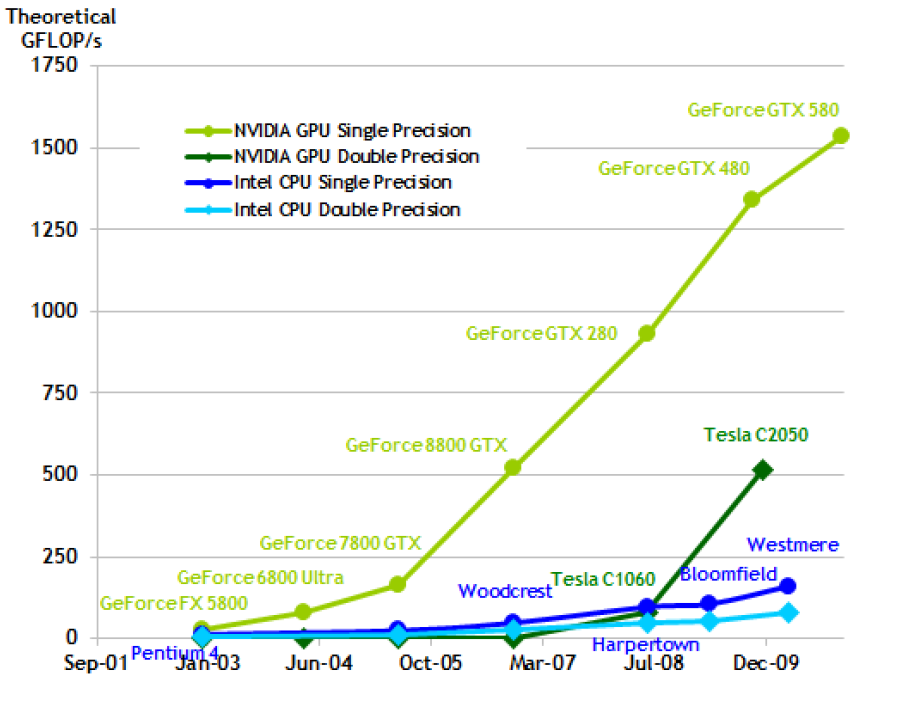
\includegraphics[width=100mm, keepaspectratio]{figures/cpower.png}
\caption{Számítási teljesítémény növekedése} 
%\label{fig:equivTV}
\end{figure}
A hardware fejlesztése a párhuzamos programozás kiszolgálása felé tolódik el.
Ha egy adott modell szimulátora megengedi a párhuzamos program futtatást, akkor az nagy
futási idő javulást jelent,
persze ezt a programkód elkészítésének bonyolultságával fizetjük meg. 
Míg eddig elég volt csupán egy magas szintű programozási nyelvet ismerni,
a GPU-k használata során az embernek mélyebben bele kell magát ásnia az architektúrájába.



\section{Architektúra és programozása}

A CUDA és az nvcc fordító lehetővé teszi adott C kód
egy részének futtatását egy átlagos PC-n
míg másik részét SIMT (single instruction, multiple thread) utasításokra fordítva
a GPU-n futtatni.
A továbbiakban a hosztnak a CPU-t, eszköznek a GPU-t fogom hívni.

\begin{figure}[H]
\centering
%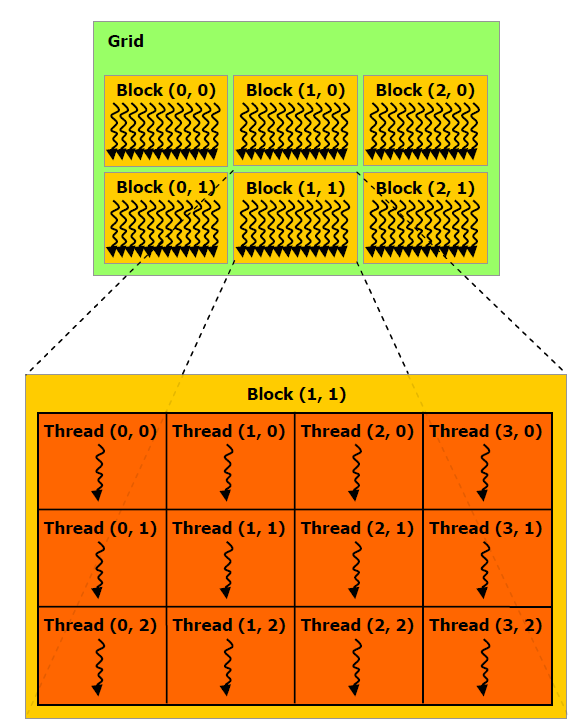
\includegraphics[width=100mm, keepaspectratio]{figures/cudagrid.png}
\caption{A CUDA blokkszervezése} 
%\label{fig:equivTV}
\end{figure}

\noindent A CUDA szálaknak saját programszámlálójuk és regisztereik vannak.
Mindegyik szál eléri a "global memory" címteret.
Azonos blokkban lévő szálak közös "shared memory" címteren osztoznak, ami méretileg korlátozott, viszont relatíve gyors.
Blokkon belüli szálak párhuzamosan hajtódnak végre, amikor valamelyik elágazáshoz ér,
akkor onnantól kezdve sorosan folytatódik a programvégrahajtás.
Ezt követő szinkronizálás után újra párhuzamosan folytatódik a programvégrahajtás.\\


A laptopomban lévő NVIDIA GT 330M eszköznek 6 multiprocesszora egyenként 8 maggal
rendelkezik, ami 48 szál futtatását teszi lehetővé párhuzamosan.
\\

\noindent A szálakat blokkokba kell csoportosítani, egy blokk maximum 512 szálat tartalmazhat.
A blokkok egy, kettő vagy három dimenziósak is lehetnek kívánalom szerint.
\\

\noindent Kernelnek hívjuk az eszközön futó kód magját, ami futtatásához specifikálni kell
a blokkok méretét és a futtatandó függvényt.
E függvény deklarálását a \texttt{\_\_global\_\_} kulcsszóval kezdjük.
A függvény hívását a hoszt fogja kezdeményezni.

\noindent Az alapvető végrehajtási folyamat:
\begin{itemize}
\item A CPU memóriájából a GPU memóriájába másoljuk a feldolgozandó kontextust
\item Betöltjük a futtatandó programot és cacheljük
\item A futás végén a GPU memóriájából a CPU memóriájába töltjük vissza
\end{itemize}
Fontos elkülöníteni a hoszt és az eszköz memóriáját. Egyik a másik felől nem érhető el.
Az eszközön való memóriafoglalásra a következő standard működésű függvények valók:
\texttt{cudaMalloc(), cudaFree(), cudaMemcpy()}.
\newpage

\section{Mintaprogram: Két vektor összegzése blokkok és szálak használatával}

Az eszközön futó kód:
\begin{lstlisting}[frame=single]  % Start your code-block

// Az eszkozon futo mag.
__global__ void add(int *a, int *b, int *c) {
    int index = threadIdx.x + blockIdx.x * blockDim.x;
    c[index] = a[index] + b[index];
}
\end{lstlisting}
A \texttt{blockIdx.x} a blokk címzésére való változó, ami érrékének állítását a fordító elrejti előlünk.

\begin{lstlisting}[frame=single]  % Start your code-block

#define T 512
#define B T*512
int main(void) {
    int *a, *b, *c;				// a, b, c hoszt peldanya
    int *d_a, *d_b, *d_c;			// a, b, c eszkoz peldanya
    int size = B * sizeof(int);
    
    // a, b, c-nek memoriafoglalas az eszkozon
    cudaMalloc((void **)&d_a, size);
    cudaMalloc((void **)&d_b, size);
    cudaMalloc((void **)&d_c, size);
    
    // a, b, c-nek memoriafoglalas a hoszton
    a = (int *)malloc(size); random_ints(a, N);
    b = (int *)malloc(size); random_ints(b, N);
    c = (int *)malloc(size);
    
    // Az adatok masolasa az eszkozre
    cudaMemcpy(d_a, a, size, cudaMemcpyHostToDevice);
    cudaMemcpy(d_b, b, size, cudaMemcpyHostToDevice);
    
    // A mag futtatasa B blokkon es blokkonkent T szalon
    add<<<B,T>>>(d_a, d_b, d_c);
    
    // Az eredmeny visszamasolasa
    cudaMemcpy(c, d_c, size, cudaMemcpyDeviceToHost);
    
    free(a); free(b); free(c);
    cudaFree(d_a); cudaFree(d_b); cudaFree(d_c);
    return 0;
}
\end{lstlisting}

















